\usetikzlibrary{quotes}
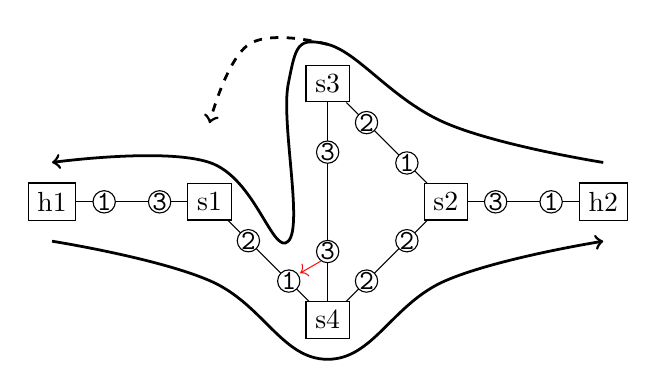
\begin{tikzpicture}
    \tikzstyle{host}=[draw]
    \tikzstyle{switch}=[draw]
    \tikzstyle{connection}=[]
    \tikzstyle{constr}=[right,font=\ttfamily\small]
    \tikzset{every edge quotes/.style={fill=white,draw, circle,inner sep=0pt}}
\node (h1) [host] at (-0.5,0.5) {h1};
\node (s1) [switch] at (1.5,0.5) {s1};
\node (s3) [switch] at (3,2) {s3};
\node (s2) [switch] at (4.5,0.5) {s2};
\node (s4) [switch] at (3,-1) {s4};
\node (h2) [host] at (6.5,0.5) {h2};
\ttfamily
\draw  (h1) edge ["1" near start, "3" near end] (s1);
% \draw  (s1) edge ["1" near start, "1" near end] (s3);
\draw  (s3) edge ["2" near start, "1" near end] (s2);
\draw  (s2) edge ["2" near start, "2" near end] (s4);
\draw  (s4) edge ["1" near start, "2" near end] (s1);
\draw  (s2) edge ["3" near start, "1" near end] (h2);
\draw  (s3) edge ["3" near start, "3" near end] (s4);
\draw[->,line width=1pt]  plot[smooth, tension=.7] coordinates {(-0.5,0) (1.5,-0.5) (3,-1.5) (4.5,-0.5) (6.5,0)};
\draw[->,line width=1pt]  plot[smooth, tension=.7] coordinates {(6.5,1) (4.5,1.5) (3,2.5) (2.5,2) (2.5,0) (1.5,1) (-0.5,1)};
\draw[->,dashed,line width=1pt]  plot[smooth, tension=.7] coordinates {(3,2.5) (2,2.5) (1.5,1.5)};
\node[red,rotate=30] at (2.8,-0.35) {$\leftarrow$};
\end{tikzpicture}